The Standard Model (SM) is the most successful theory for describing elementary particles and their interactions via the electromagnetic, strong, and weak forces in terms of gauge theory interactions. The existence of an additional U(1) hidden symmetry is not forbidden by the SM. The heavy photon is the proposed gauge boson for the dark electromagnetic force that would arise from a U(1) broken symmetry. If such an interaction exists, then the SM photon and heavy photon would mix, thus inducing a coupling between the heavy photon and electric charge equal to $\epsilon e$~\cite{holdom_two_1986}. This coupling is significant because electrons could radiate heavy photons similar to radiating SM photons, although at rates decreased by $\epsilon^2$. The primary goal of HPS and many similar experiments is to experimentally detect the heavy photon through this production mechanism. The heavy photon is additionally referred to as the $A^{\prime}$, dark photon, or $U-$boson.

\section{Theory of heavy photons}
The possible existence of a heavy photon rests on the allowable symmetries from the Standard Model. An additional U(1) symmetry in nature could interact with the SM through the mechanism of kinetic mixing~\cite{holdom_two_1986}. Under kinetic mixing, a new gauge boson (heavy photon or $A^{\prime}$ couples to the electromagnetic current through the SM photon by some amount $\epsilon$. Kinetic mixing generates the coupling strength, $\epsilon$, through loop interactions as shown in Figure~\ref{fig:loop}. 

\begin{figure}[htb]
    \begin{center}
        \begin{fmffile}{loop}
            \begin{fmfgraph*}(150,150)
                \fmfstraight 
                \fmfleft{i1}
                \fmfright{o1}
                \fmflabel{$\gamma$}{i1}
                \fmflabel{$A'$}{o1}
                \fmf{photon,tension=1}{i1,v1}
                \fmf{photon,tension=1}{v2,o1}
                \fmf{fermion,left,label=$\chi$}{v2,v1}
                \fmf{fermion,left,label=$\chi^{\prime}$}{v1,v2}
            \end{fmfgraph*}
        \end{fmffile}
    \end{center}
    \caption[Kinetic mixing of the SM photon with a heavy photon]{Kinetic mixing of the SM photon with a heavy photon is shown at the one-loop level. $\chi$ can be any massive particle that is charged under both the $A^{\prime}$ and SM U(1) interactions.}
    \label{fig:loop}
\end{figure}

In the simplest scenario, there is one particle $\chi$ that is charged under both the U(1) and new U(1)$^{\prime}$. This single loop level interaction can generate the $\epsilon$ coupling to be in the range of $10^{-2}$ to $10^{-4}$. In Grand Unified Theory (GUT), symmetries forbid one-loop interactions and favor two-loop interactions generating an $\epsilon$ in the range of $10^{-3}$ to $10^{-5}$~\cite{alexander_dark_2016}. If both U(1)s are in unified groups, higher loop interactions generating even smaller couplings are possible. The gauge part of the SM Lagrangian is modified to include this interaction

\begin{equation}
	\label{eq:lagrangian}
\mathcal{L}_{gauge} = -\dfrac{1}{4}F^{\mu\nu}F_{\mu\nu}-\dfrac{1}{4}
F^{\prime\mu\nu}F^{\prime}_{\mu\nu}-\dfrac{1}{2}\epsilon F^{\mu\nu}F^{\prime}_{\mu\nu}
\end{equation}
where $F_{\mu\nu}$ is the electromagnetic field strength tensor defined in terms of the gradient of the potential as $F_{\mu\nu}=\partial_{\mu}A_{\nu}-\partial_{\nu}A_{\mu}$, $F^{\prime}_{\mu\nu}$ corresponds to the field strength of the heavy photon, and $\epsilon$ is the coupling. The third term of the Lagrangian is the kinetic mixing operator. The SM photon field can be re-defined as $A_{\mu}\rightarrow A_{\mu}+\epsilon A^{\prime}_{\mu}$ to remove the kinetic mixing operator. This generates a coupling to electric charge of order $\epsilon$ seen in the interaction between the heavy photon and SM as $\epsilon e A^{\prime}_{\mu}J^{\mu}_{EM}$ where $J^{\mu}_{EM}$ is the electromagnetic current~\cite{bjorken_new_2009}. Particles that are charged only under the $A^{\prime}$ would not acquire this fractional charge and would remain undetectable in this model. \\
\indent The mass of the heavy photon is somewhat less constrained by theory. The MeV to GeV mass scale is interesting to explore because it has been generally overlooked by previous experiments and is consistent with dark matter theories that attempt to explain several astrophysical observations. 


\section{Implications of a heavy photon}
The theory for the existence of the heavy photon arises from allowable symmetries of the Standard Model and can exist without other theories of dark matter. However, if the heavy photon does exist, then the interaction between the heavy photon and the Standard Model through the vector portal could be  the leading interaction between the Standard Model and the Dark Sector (where the Dark Sector comprises the dark energy and dark matter which we can only observe indirectly through gravitational effects).

\subsection{Mediator of dark matter interactions}

Astrophysical observations of the rotational velocity of spiral galaxies has indicated the large presence of an unidentifiable mass contribution~\cite{Sofue:2000jx}. The simplest model to explain this additional mass contribution, Lambda Cold Dark Matter ($\Lambda$CDM), estimates that nearly one-third of the universe is composed of this dark matter while SM particles only compose some 4$\%$ of the universe. $\Lambda$CDM is consistent with measurements of the Cosmic Microwave Background (CMB) power spectrum which indicates the relative quantities of dark matter and SM matter~\cite{madhavacheril_current_2014}. The theory of $\Lambda$CDM requires no force beyond that of gravity for dark matter particles (``collisionless" dark matter), but discrepancies between simulation and observations indicate that the theory is still incomplete~\cite{weinberg_cold_2013}. In particular, collisionless dark matter simulations generate cuspy dark matter halos with a changing density and velocity profile as well as halos containing significant structure. However, astrophysical observations indicate that the cores are of constant density and only a handful of subhalos have been observed in the Milky Way.  \\
\indent Weakly Interacting Massive Particles (WIMPs) have been a prime dark matter candidate for several decades with particles in the 10s of GeV to TeV mass range and interaction strengths characterized by the weak scale. While many experiments have been devoted to the detection of WIMPs through nuclear recoils and missing energy measurements, no confident signal has been detected~\cite{liu_signals_2015}. Light dark matter with masses in the MeV to GeV range are strongly motivated as a theory that has been previously overlooked but could explain various astrophysical phenomena. In order to have the correct relic abundance in a theory of light dark matter, a new force is required to mediate dark matter interactions. The presence of a new boson force carrier can suppress the dark matter annihilation cross sections through a Somerfeld enhancement~\cite{arkani-hamed_theory_2009} and can only happen if the gauge boson has a mass of GeV scale and smaller. The Somerfeld enhancement boosts the annihilation cross section at lower velocities and yields the correct thermal relic abundance. \\

\subsection{Observations for light dark matter}
An eXciting Dark Matter (XDM) model proposes that dark matter can scatter via a heavy photon into excited states that can subsequently decay into  dark matter and a SM photon~\cite{finkbeiner_x-ray_2014}. This process is shown in Figure~\ref{fig:excitation}.

\begin{figure}[htb]
    \begin{center}
	\begin{fmffile}{excitedDM}
	\begin{fmfgraph*}(150,150)
	\fmfleft{i1,i2}
	\fmfright{o1,o2}
	\fmflabel{$\chi$}{i1}
	\fmflabel{$\chi$}{i2}
	\fmflabel{$\chi^{\ast}$}{o1}
	\fmflabel{$\chi^{\ast}$}{o2}			
	\fmf{fermion}{i1,v1,o1}
	\fmf{fermion}{i2,v2,o2}
	\fmf{photon,label=$A'$}{v1,v2}
\end{fmfgraph*}
	\end{fmffile}
  	\end{center}
    	\caption[Heavy photon mediates dark matter scattering into an excited state]{The heavy photon mediates dark matter scattering into an excited state. Excited dark matter could subsequently decay producing observable X-ray emission spectra $\chi^{\ast}\rightarrow\chi\gamma$.}
   	 \label{fig:excitation}	
\end{figure}

This model could account for the observed 3.5~keV X-ray emission line observed in 73 galaxy clusters~\cite{bulbul_detection_2014}. The cores of galaxies are of interest to study and look for signals of dark matter interactions.  Additionally, observations of a gamma ray excess around the Galactic Center cannot be explained through known processes of interactions with cosmic rays and gamma rays from known sources~\cite{Hooper:2010mq}. This observation can be further explained through a model involving light dark matter interactions. 

\subsection{Historical motivators}
Astrophysical anomalies and tests of the SM have been historical motivators to explore a theory of light dark matter with a dark force mediator. \\
\indent An excess in the positron fraction measured in cosmic rays was detected above 10~GeV by several different balloon payload experiments including HEAT~\cite{Barwick:1995gv} and CAPRICE~\cite{Boezio:2001dtm} and confirmed in space telescopes such as PAMELA~\cite{adriani_observation_2009}, the Fermi Large Area Telescope~\cite{Abdollahi:2017nat}, and the Alpha Magnetic Spectrometer~\cite{Schael:2007tta}. Positrons are known to be produced in interactions between cosmic ray nuclei and interstellar matter, but the excess was unforeseen from these sources alone. Alternatively, the measured anti-proton spectrum did not show an excess in the spectrum and was consistent with these secondary processes. These phenomena motivated a theory of light dark matter scattering mediated by a heavy photon with a mass $<2m_p$ that could decay to lepton pairs. Further measurements of the positron spectrum from the AMS-02 should have yielded a bump in the positron excess at higher energies if the lepton pairs were the result of a heavy photon decay. As no apparent bump in this spectrum was observed~\cite{Bergstrom:2013jra}, the data from AMS-02 is used to constrain theories of light dark matter~\cite{liu_signals_2015}. \\
\indent The muon anomalous magnetic moment, $g-2$, was measured as having a larger than three standard deviation discrepancy than what is predicted by the SM~\cite{blum_muon_2013}. This difference could be accounted for if there is an additional contribution from a heavy photon correction. Several experiments ruled out the possibility of a heavy photon that decays visibly being able to account for this effect, but a heavy photon that decays invisibly is still possibly responsible for this effect. The contribution from a heavy photon interaction to the muon $g-2$ is shown in Figure~\ref{fig:gm2}.

\begin{figure}[ht]
    \begin{center}
        \begin{fmffile}{gm2}
            \begin{fmfgraph*}(150,150)
                \fmfstraight 
                \fmftop{o1}
                \fmfbottom{i1,i2}
                \fmflabel{$\mu$}{i1}
                \fmflabel{$\mu$}{i2}
                \fmf{fermion}{i1,v1,v2,v3,i2}
                \fmf{photon,label=$\gamma$}{v2,o1}
                \fmffreeze
                \fmf{photon,label=$A'$}{v1,v3}
            \end{fmfgraph*}
        \end{fmffile}
    \end{center}
    \caption{Heavy photon contribution to the muon $g-2$.}
    \label{fig:gm2}
\end{figure}

\section{Searching for heavy photons}
Due to the mechanism of kinetic mixing, the production of the heavy photon is similar to that of a photon radiating from an electron although at a suppressed rate proportional to the coupling $\epsilon^2$. The final states into which the heavy photon can decay is related to the model of the dark sector and corresponding dark matter mass $m_{\chi}$. A heavy photon that is heavier than $2m_{\chi}$ can decay into completely invisible states or a mixture of invisible states and SM states. Here, we focus solely on the scenario of a heavy photon that decays visibly to SM particles (this also implies that the heavy photon is lighter than twice the lightest dark matter mass). 

\subsection{Decay signature}
The branching ratio of the heavy photon is obtained from the ratios of different final state measurements of $e^+e^-\rightarrow $ hadrons at various center-of-mass energies~\cite{liu_signals_2015}. In the mass regime that HPS explores, the heavy photon will decay to $e^+e^-$ pairs as shown in Figure~\ref{Figure:br}. 

\begin{figure}[htb]
  \centering
      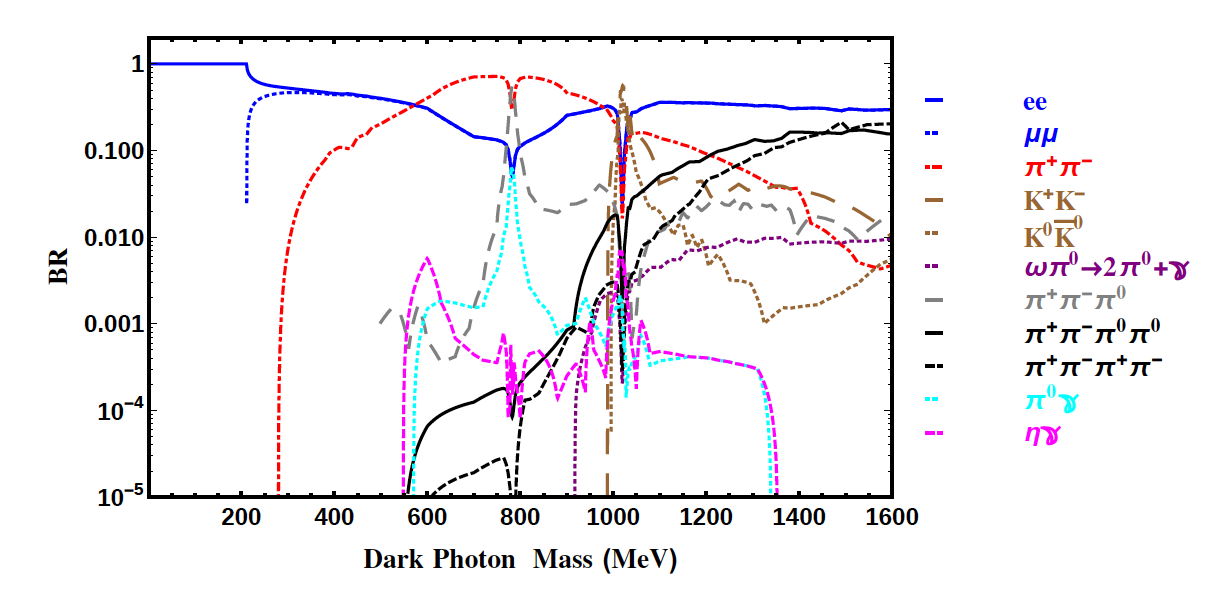
\includegraphics[width=0.9\textwidth]{pics/motivation/branchingRatio.png}
 	 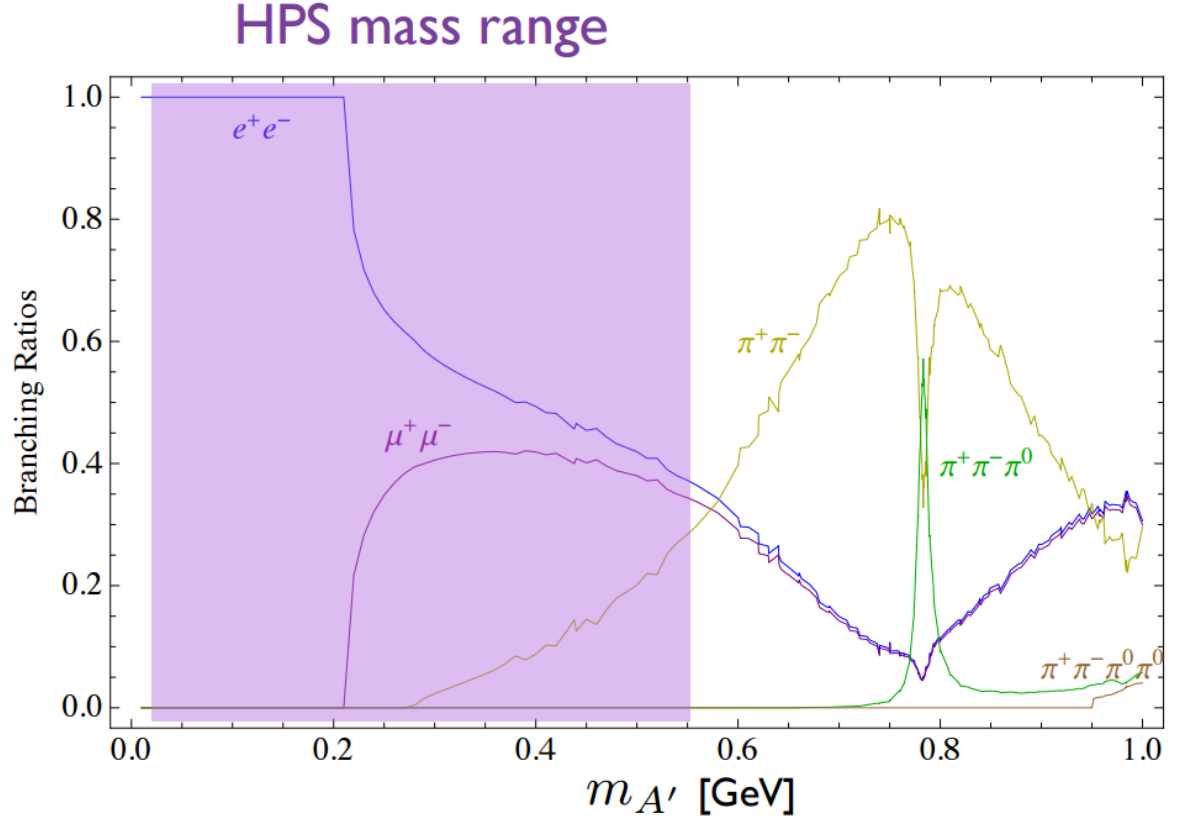
\includegraphics[width=0.5\textwidth]{pics/motivation/branchingLinear.png}	
  \caption[The branching fraction ratios for heavy photon decays]{The branching fraction ratios for heavy photons of various masses is shown~\cite{liu_signals_2015}. The top plot is shown for an extended mass range and log scale whereas the bottom plot shows a more limited mass range and linear scaling. The mass range that HPS is most sensitive to is highlighted in purple in the bottom plot.}
  \label{Figure:br}
\end{figure}

HPS searches for heavy photons of masses 20 to 100~MeV/c$^2$. As shown in Figure~\ref{Figure:br}, at heavy photon masses above 200~MeV/c$^2$, the branching ratio for decays to $e^+e^-$ decreases sharply and decays to $\mu^+\mu^-$ becomes significant. \\
\indent Assuming that the heavy photon only decays to SM final states, the proper lifetime of the $A^{\prime}$ neglecting phase space corrections is described by   

\begin{equation}
	\label{eq:propLife}
	\begin{split}
	c\tau &= \dfrac{1}{\Gamma}\simeq \dfrac{3}{N_{eff}m_{A^{\prime}}\alpha\epsilon^2}\\
	&\simeq \dfrac{0.8\textrm{ cm}}{N_{eff}}\Big({\dfrac{10^{-4}}{\epsilon}}\Big)^2\Big(\dfrac{100\textrm{ MeV}}{m_{A^{\prime}}}\Big)
	\end{split}
\end{equation}
where $N_{eff}$ is the number of available decay states ($=1$ at $m_{A^{\prime}}<2m_{\mu}$)~\cite{bjorken_new_2009}. The lifetime is inversely proportional to the coupling $\epsilon^2$. For small couplings, the heavy photon will travel a measurable distance before decaying. The decay length is 

\begin{equation}
	\label{eq:decayL}
	\begin{split}
	l_0 &\equiv \gamma c \tau \\
	&\simeq \dfrac{0.8\textrm{ cm}}{N_{eff}}\Big(\dfrac{E_{beam}}{10\textrm{ GeV}}\Big)\Big({\dfrac{10^{-4}}{\epsilon}}\Big)^2\Big(\dfrac{100\textrm{ MeV}}{m_{A^{\prime}}}\Big)^2
	\end{split}
\end{equation}
where $E_{beam}$ is the incident electron energy. The rate of $A^{\prime}$ production is dependent on $\alpha^3\epsilon^2/m_{A^{\prime}}^2$ and is suppressed relative to ordinary bremsstrahlung by a factor of $\epsilon^2m_{e-}^2/m_{A^{\prime}}^2$~\cite{bjorken_new_2009}. The ratio of the fully differential production cross sections for the heavy photon relative to the production of a virtual photon is:

\begin{equation}
	\label{eq:production}
	\dfrac{d\sigma(e^-Z\rightarrow e^-ZA^{\prime}\rightarrow e^-Zl^+l^-)}{d\sigma(e^-Z\rightarrow e^-Z\gamma^{\ast}\rightarrow e^-Zl^+l^-)} = \Big(\dfrac{3\pi\epsilon^2}{2N_{eff}\alpha}\Big) \Big(\dfrac{m_{A^{\prime}}}{\delta m_{A^{\prime}}}\Big)
\end{equation}
This ratio represents the maximum signal to background that can be achieved in an experiment. The heavy photon is produced at very forward, small angles and carries nearly all of the beam energy. \\

\subsection{Methods of production}
Heavy photons can be produced experimentally in fixed-target experiments and collider experiments. Fixed-target experiments are complementary to collider experiments in that they can generally access smaller coupling due to the high luminosity while collider experiments can probe higher heavy photon masses due to the higher center of mass energy attainable. In electron fixed-target experiments, the heavy photon is generated through a bremsstrahlung-like process and is detected from the final state particles. Proton fixed-target experiments look for the signal in the decay products of various mesons produced from the beam interaction with the target. Looking for heavy photons produced in meson decays such as Dalitz decays ($\pi^0, \eta, \eta^{\prime}\rightarrow \gamma A^{\prime}$), ($K\rightarrow\pi A^{\prime} $, $\phi\rightarrow\eta A^{\prime}$, and $D^{\ast}\rightarrow D^{0}A^{\prime}$) are another production mechanism that has been used at both colliders and fixed target-type experiments. Drell-Yan ($q\bar{q}\rightarrow A^{\prime}$) experiments are more common at proton fixed target and hadron collider experiments. Both $e^+e^-$ colliders and hadron colliders search for heavy photons in the decay channels shown in Figure~\ref{Figure:br} and are particularly well-suited to search for heavy photons that decay invisibly due to their ability to precisely reconstruct the initial state. 

\subsection{Methods of detection}

The strategies for searching for heavy photons are typically a bump hunt on the visible final state particles, a bump hunt in the missing mass spectrum (for invisible decays), or a detached vertex search for heavy photons with small couplings. \\
\indent Electron fixed-target experiments produce heavy photons through bremsstrahlung-like processes with the electron beam incident on a heavy target. Heavy photons are produced in a very forward direction requiring high resolution spectrometers or detectors close to the beam. Previous limits set by this type of experiment include the A1 experiment that uses the Microtron beam at Mainz and the A1 high resolution spectrometer to reconstruct the $e^+e^-$ pair~\cite{beranek_theoretical_2013}. The A1 experiment significantly ruled out parameter space where the heavy photon was a possible explanation to resolve the muon $g-2$ anomaly. The APEX experiment at Jefferson Lab Hall A produced electron bremsstrahlung and used the high resolution spectrometers to measure the $e^+e^-$ particles~\cite{abrahamyan_search_2011}. APEX performed a bump hunt on the final state particles in the mass range 65-600~MeV and will likely take data again in 2018. DarkLight is another Jefferson Lab experiment that places a windowless gas target in the Low Energy Recirculator Facility using a 100~MeV beam to search for heavy photons with low masses. DarkLight will perform a bump hunt search in the $e^+e^-$ mass spectrum and may have some ability to search for invisible decays by using a silicon layer to detect proton recoils~\cite{balewski_darklight_2014}.\\
\indent Proton fixed target experiments look for heavy photons in the decays of particles produced from beam interaction at the target. The NA48/2 experiment at the CERN SPS produced $K^{\pm}$ beams and searched for heavy photons from the $\pi^0$ decay produced from the in-flight decay of the $K^{\pm}$~\cite{Batley_2015lha}. SHiP is a future experiment at the CERN SPS that will use a 400~GeV proton beam to look in both Drell Yan and meson decays for heavy photons. SHiP will be sensitive to long decay lengths (on the order of 10s of meters) and will cover a wide mass range in visible decay states up to 10~GeV masses. SHiP is expected to run sometime after 2026~\cite{ship_collaboration_facility_2015}.\\
\indent Beam dump experiments look for heavy photons with long decay lengths. The beam dump experiments E141 and E137 at SLAC, E774 at Fermilab, and one at Orsay were originally run to look for MeV-mass axion-type particles from electron beam dumps~\cite{alexander_dark_2016}. The U70 beam dump looked for heavy photons downstream from a proton beam on a fixed target~\cite{Blumlein:2013cua}. SeaQuest at Fermilab looks for muon pairs produced downstream from the 120~GeV proton beam on a fixed target. It is speculated that by analyzing previous data taken (E906/SeaQuest), a 95$\%$ confidence limit on heavy photon masses in the range of 215-5600~MeV is possible. SeaQuest is currently establishing upgrades for improved future running~\cite{gardner_new_2016}.\\
\indent Collider experiments using $e^+e^-$ or $pp$ collisions complement the fixed-target experiments and are favored for looking for heavy photon invisible decays.  BaBar, an experiment at the Stanford Linear Accelerator (SLAC) $e^+e^-$ collider, set limits by searching for the $A^{\prime}$ in missing mass around the $\Upsilon(2S)$, $\Upsilon(3S)$, and $\Upsilon(4S)$ resonances~\cite{Lees_2014xha}. In the near future, LHCb at CERN is expected to look for heavy photons in the di-muon invariant mass spectrum from rare heavy quark decays produced from proton-proton collisions. LHCb will be sensitive to the heavy photons with both prompt and displaced vertices and is expected to run sometime after 2021~\cite{Ilten_2016tkc}. The limits established by existing searches can be seen in Figure~\ref{Figure:projReach}.

\section{Heavy Photon Search kinematics}
The HPS experiment sends an electron beam through a thin tungsten target and looks for radiated heavy photons in the reconstructed $e^+e^-$ mass spectrum. HPS looks for heavy photons in the range of 20 to 1000~MeV/c$^2$ and covers this territory with two searches on the same dataset that probe different heavy photon coupling regimes. A bump hunt searches for the heavy photon signal as a resonance on a large background. The bump hunt looks for heavy photons with large couplings and decay at the target. The vertex search looks for heavy photons that have detached vertices, having a measurable lifetime and decaying downstream of the target. 

\subsection{Signal}

The heavy photon is generated from the electron beam interaction with a heavy target as shown in Figure~\ref{fig:apTree} where $Z$ is the atomic number corresponding to the target material.  

\begin{figure}[htb]
    \begin{center}
	\begin{fmffile}{apTree}
	\begin{fmfgraph*}(150,150)
	\fmfstraight
		\fmfleft{i1,i2,i3,i4}
		\fmfright{o1,o2,o3,o4}
		\fmflabel{$Z$}{i1}
		\fmflabel{$e-$}{i2}
		\fmflabel{$e-$}{o2}
		\fmflabel{$e-$}{o3}
		\fmflabel{$e+$}{o4}	
		\fmf{heavy}{i1,v1,o1}
		\fmffreeze
		\fmf{fermion}{i2,v2,v3,o2}				
		\fmffreeze	
		\fmf{fermion}{o4,v4,o3}
		\fmf{photon,tension=0,label=$\gamma$}{v1,v2}
		\fmf{photon,tension=2,label=$A^{\prime}$}{v3,v4}
	\end{fmfgraph*}
	\end{fmffile}
  	\end{center}
    	\caption[Heavy photon production in a fixed-target experiment]{The heavy photon is produced in a process analagous to bremsstrahlung on a heavy target of atomic number $Z$.}
   	 \label{fig:apTree}	
\end{figure}

Shown for the HPS experiment, the heavy photon decays to $e^+e^-$ pairs with a measurable mass and possible displaced vertex downstream from the target. The differential cross section for heavy photon production is 

\begin{equation}
	\label{eq:apDiffCS}
	\dfrac{d\sigma}{dxd\cos\theta_{A^{\prime}}} \approx \dfrac{8Z^2\alpha^3\epsilon^2E_0^2x}{U(x,\theta_{A^{\prime}})^2}\log\Big( (1-x+\dfrac{x^2}{2})-\dfrac{x(1-x)m_{A^{\prime}}^2E_0^2x\theta_{A^{\prime}}^2}{U(x,\theta_{A^{\prime}})^2}\Big)
\end{equation}
where $Z$ is the atomic number of the target material, $\alpha$ is the usual fine structure constant, $\theta_{A^{\prime}}$ is the lab frame angle of the outgoing heavy photon, $E_0$ is the electron incident energy, $m_{A^{\prime}}$ is the heavy photon mass, and the fraction of incident beam energy carried by the the heavy photon is $x\equiv E_{A^{\prime}}/E_0$~\cite{bjorken_new_2009}. The virtuality of the intermediate electron is described by

\begin{equation}
	\label{eq:virtuality}
	U(x,\theta_{A^{\prime}}) = E_0^2x\theta_{A^{\prime}}^2+m_{A^{\prime}}^2\dfrac{1-x}{x}+m_e^2x 
\end{equation}
where $m_e$ is the mass of the electron. The cross section is further simplified for $m_e\ll m_{A^{\prime}}\ll E_0$ and $x\theta_{A^{\prime}}^2\ll 1$. Integrating Equation~\eqref{eq:apDiffCS} over the angle, the cross section is

\begin{equation}
	\label{eq:csFinal}
	\dfrac{d\sigma}{dx} \approx \dfrac{8Z^2\alpha^3\epsilon^2x}{m_{A^{\prime}}^2}\Big(1+\dfrac{x^2}{3(1-x)}\Big)
\end{equation}
The total heavy photon production rate is proportional to $\alpha^3\epsilon^2/m_{A^{\prime}}^2$ and is suppressed relative to photon bremsstrahlung by $\epsilon^2m_e^2/m_{A^{\prime}}^2$.The singularity is regulated by the mass of the electron and cutoff for values where $1-x$ exceeds $m_e^2/m_{A^{\prime}}^2$ or $m_{A^{\prime}}^2/E_0^2$. The heavy photon carries nearly the entire beam energy such that the median value of $1-x\sim\textrm{max}\Big(\dfrac{m_e}{m_{A^{\prime}}}, \dfrac{m_{A^{\prime}}}{E_0}\Big)$. The heavy photon is emitted predominately at small angles with a cutoff at $\dfrac{m_{A^{\prime}}^{3/2}}{E_0^{3/2}}$ such that the angular emission falls off as $1/\theta_{A^{\prime}}^4$.\\
 \indent The heavy photon is characterized by its mass (as reconstructed from the decay to $e^+e^-$) and decay length. Depending on the coupling strength $\epsilon$, the vertex may be reconstructed from a prompt decay at the target or a measurable decay downstream.  

\subsection{Backgrounds}

The primary backgrounds in this experiment include trident events and wide angle bremsstrahlung (WAB). The tridents have the same three particle final state $e^-e^-e^+$ and are broadly categorized into radiative and Bethe-Heitler diagrams~\cite{bjorken_new_2009}. The trident events were the primary source of background considered prior to running the experiment. It was later found that WAB events contributed to the background with an $e^-\gamma$ final state where the photon then produced an $e^+e^-$. In most cases, the event was triggered by the initial electron and pair-produced positron. 

\begin{figure}[htb]
    \begin{center}
	\begin{fmffile}{radTree}
	\begin{fmfgraph*}(150,150)
	\fmfstraight
		\fmfleft{i1,i2,i3,i4}
		\fmfright{o1,o2,o3,o4}
		\fmflabel{$Z$}{i1}
		\fmflabel{$e-$}{i2}
		\fmflabel{$e-$}{o2}
		\fmflabel{$e-$}{o3}
		\fmflabel{$e+$}{o4}	
		\fmf{heavy}{i1,v1,o1}
		\fmffreeze
		\fmf{fermion}{i2,v2,v3,o2}				
		\fmffreeze	
		\fmf{fermion}{o4,v4,o3}
		\fmf{photon,tension=2,label=$\gamma$}{v1,v2}
		\fmf{photon,tension=2,label=$\gamma$}{v3,v4}
	\end{fmfgraph*}
	\end{fmffile}
  	\end{center}
    	\caption[Radiative background]{Radiative trident background process: The photon is radiated from the electron incident on a heavy target of atomic number $Z$ and produces and $e^+e^-$ pair. The radiatives have the same kinematics as the heavy photon and comprise the primary background in the bump hunt analysis where all decays are prompt. }
   	 \label{fig:radTree}	
\end{figure}

The radiative background is irreducible and comprises the smooth background upon which the bump hunt search for the heavy photon signal is conducted. The Bethe-Heitler tridents also contribute significantly to the background although they are peaked at lower $e^+e^-$ total energy. The Bethe-Heitler contribution is shown in Figure~\ref{fig:bhTree}.

\begin{figure}[htb]
    \begin{center}
	\begin{fmffile}{bhTree}
	\begin{fmfgraph*}(150,150)
	\fmfstraight
		\fmfleft{i1,i2,i3,i4}
		\fmfright{o1,o2,o3,o4}
		\fmflabel{$Z$}{i1}
		\fmflabel{$e-$}{i4}
		\fmflabel{$e-$}{o2}
		\fmflabel{$e+$}{o3}
		\fmflabel{$e-$}{o4}	
		\fmf{heavy}{i1,v1,o1}
		\fmffreeze
		\fmf{fermion}{i4,v4,o4}				
		\fmffreeze	
		\fmf{photon,tension=1,label=$\gamma$}{v1,v2}
		\fmf{photon,tension=1,label=$\gamma$}{v3,v4}
		\fmf{fermion}{o3,v3,v2,o2}
	\end{fmfgraph*}
	\end{fmffile}
  	\end{center}
    	\caption[Bethe-Heitler background]{Bethe-Heitler trident background process: The photon produced from electron interaction at a target of atomic number $Z$ produces an $e^+e^-$ pair that often have a total energy much less than the initial beam energy. The recoil electron and the Bethe-Heitler positron can also be detected.}
   	 \label{fig:bhTree}	
\end{figure}

The radiative and Bethe-Heitler diagrams also interfere although this generally only contributes at lower $e^+e^-$ total energy. 